\documentclass{article}

\usepackage{amsmath}
\usepackage{amssymb}
\usepackage{tikz}
\usepackage{xcolor}

\usetikzlibrary{positioning, calc, shapes.symbols} 

\title{Intermediate Axis Theorem}
\author{finegeometer}

\begin{document}
\maketitle

Throughout this article, I describe linear-algebraic concepts in graphical notation.
To avoid confusion, I use \textcolor{blue}{blue} wires to represent vectors in the body frame,
and \textcolor{red}{red} to represent vectors in the fixed frame.

\vspace*{1em}\hrule\vspace*{1em}

Consider a rigid body, made of masses \(m_\alpha\) at locations
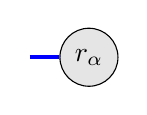
\begin{tikzpicture}[baseline={([yshift=-.5ex]current bounding box.center)}]
    \node[circle,draw,fill=gray!20] (a) at (0.75,0) {\(r_\alpha\)};
    \draw[blue, ultra thick] (0,0) -- (a);
\end{tikzpicture}
relative to the center of mass.
We allow it to rotate freely, but fix its center of mass to the origin.

How do we represent the state of the system? The thing that's changing over time is the object's orientation.
This is equivalently \emph{the relationship between the body frame and the fixed frame.}

This relationship is an isometry, hence an affine transformation.
Since it maps the origin of the body frame to the origin of the fixed frame,
it's a linear transformation. I call it
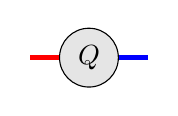
\begin{tikzpicture}[baseline={([yshift=-.5ex]current bounding box.center)}]
    \node[circle,draw,fill=gray!20] (a) at (0,0) {\(Q\)};
    \draw[red, ultra thick] (a) -- (-0.75,0);
    \draw[blue, ultra thick] (a) -- (0.75,0);
\end{tikzpicture},
since it's our ``position'' coordinate.

In fact, it should be an \emph{orthogonal} linear transformation. So we impose a constraint:
\(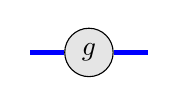
\begin{tikzpicture}[baseline={([yshift=-.5ex]current bounding box.center)}]
    \node[circle,draw,fill=gray!20] (a) at (0,0) {\(g\)};
    \draw[blue, ultra thick] (a) -- (-0.75,0);
    \draw[blue, ultra thick] (a) -- (0.75,0);
\end{tikzpicture} \stackrel{\text{def}}{=} 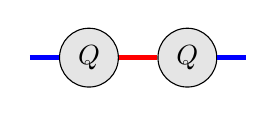
\begin{tikzpicture}[baseline={([yshift=-.5ex]current bounding box.center)}]
    \node[circle,draw,fill=gray!20] (a) at (0.75,0) {\(Q\)};
    \node[circle,draw,fill=gray!20] (b) at (2,0) {\(Q\)};
    \draw[blue, ultra thick] (0,0) -- (a);
    \draw[red, ultra thick] (a) -- (b);
    \draw[blue, ultra thick] (b) -- (2.75,0);
\end{tikzpicture} - 
\begin{tikzpicture}[baseline={([yshift=-.5ex]current bounding box.center)}]
    \draw[blue, ultra thick] (0,0) -- (0.75,0);
\end{tikzpicture} = 0\),

\vspace*{1em}\hrule\vspace*{1em}

We apply Lagrangian mechanics.

In the fixed frame, the position of the mass \(m_\alpha\) is 
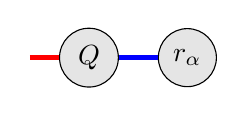
\begin{tikzpicture}[baseline={([yshift=-.5ex]current bounding box.center)}]
    \node[circle,draw,fill=gray!20] (a) at (0.75,0) {\(Q\)};
    \node[circle,draw,fill=gray!20] (b) at (2,0) {\(r_\alpha\)};
    \draw[red, ultra thick] (0,0) -- (a);
    \draw[blue, ultra thick] (a) -- (b);
\end{tikzpicture},
so the velocity is
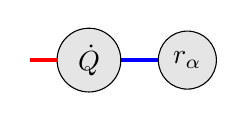
\begin{tikzpicture}[baseline={([yshift=-.5ex]current bounding box.center)}]
    \node[circle,draw,fill=gray!20] (a) at (0.75,0) {\(\dot{Q}\)};
    \node[circle,draw,fill=gray!20] (b) at (2,0) {\(r_\alpha\)};
    \draw[red, ultra thick] (0,0) -- (a);
    \draw[blue, ultra thick] (a) -- (b);
\end{tikzpicture}.
Therefore, the kinetic energy of the rigid body is:
\[\sum_\alpha \frac{m_\alpha}{2}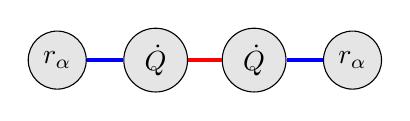
\begin{tikzpicture}[baseline={([yshift=-.5ex]current bounding box.center)}]
    \node[circle,draw,fill=gray!20] (a) at (0,0) {\(r_\alpha\)};
    \node[circle,draw,fill=gray!20] (b) at (1.25,0) {\(\dot{Q}\)};
    \node[circle,draw,fill=gray!20] (c) at (2.5,0) {\(\dot{Q}\)};
    \node[circle,draw,fill=gray!20] (d) at (3.75,0) {\(r_\alpha\)};
    \draw[blue, ultra thick] (a) -- (b);
    \draw[red, ultra thick] (b) -- (c);
    \draw[blue, ultra thick] (c) -- (d);
\end{tikzpicture}\]

Since there is no potential, the Lagrangian is the same.

It will be useful to write this in a slightly different form:
\[\mathcal{L} = \frac{1}{2} 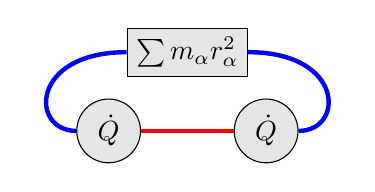
\begin{tikzpicture}[baseline={([yshift=-.5ex]current bounding box.center)}]
    \node[circle,draw,fill=gray!20] (a) at (0,0) {\(\dot{Q}\)};
    \node[circle,draw,fill=gray!20] (b) at (2,0) {\(\dot{Q}\)};
    \node[draw,fill=gray!20] (c) at (1,1) {\(\sum m_\alpha r_\alpha^2\)};
    \draw[ultra thick, red] (a) -- (b);
    \draw[ultra thick, blue] (a) .. controls +(-1,0) and +(-2,0) .. (c);
    \draw[ultra thick, blue] (b) .. controls +(1,0) and +(2,0) .. (c);
\end{tikzpicture}\]

\pagebreak

The constrained Euler-Lagrange equations says the following holds for some unknown time-dependent matrix \(\Lambda\).
\[
    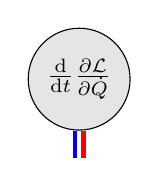
\begin{tikzpicture}[baseline=-.5ex]
        \node[circle,draw,fill=gray!20] (a) at (0,0) {\(\frac{\mathrm{d}}{\mathrm{d}t}\frac{\partial\mathcal{L}}{\partial \dot{Q}}\)};
        \draw[blue, ultra thick, transform canvas={xshift=-1.5pt}] (a) -- +(0,-1);
        \draw[red, ultra thick, transform canvas={xshift=1.5pt}] (a) -- +(0,-1);
    \end{tikzpicture}
    -
    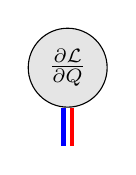
\begin{tikzpicture}[baseline=-.5ex]
        \node[circle,draw,fill=gray!20] (a) at (0,0) {\(\frac{\partial\mathcal{L}}{\partial Q}\)};
        \draw[blue, ultra thick, transform canvas={xshift=-1.5pt}] (a) -- +(0,-1);
        \draw[red, ultra thick, transform canvas={xshift=1.5pt}] (a) -- +(0,-1);
    \end{tikzpicture}
    =
    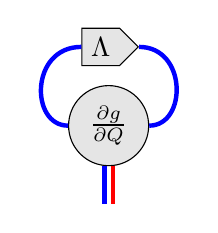
\begin{tikzpicture}[baseline=-.5ex]
        \node[circle,draw,fill=gray!20] (a) at (0,0) {\(\frac{\partial g}{\partial Q}\)};
        \node[signal,draw,fill=gray!20] (l) at (-0.1,1) {\(\Lambda\)};
        \draw[blue, ultra thick, transform canvas={xshift=-1.5pt}] (a) -- +(0,-1);
        \draw[red, ultra thick, transform canvas={xshift=1.5pt}] (a) -- +(0,-1);
        \draw[blue, ultra thick] (a) .. controls (-1,0) and (-1,1) .. (l) .. controls (1,1) and (1,0) .. (a);
    \end{tikzpicture}
\]

Evaluating the derivatives:
\begin{align*}
    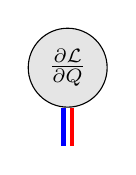
\begin{tikzpicture}[baseline=-.5ex]
        \node[circle,draw,fill=gray!20] (a) at (0,0) {\(\frac{\partial\mathcal{L}}{\partial Q}\)};
        \draw[blue, ultra thick, transform canvas={xshift=-1.5pt}] (a) -- +(0,-1);
        \draw[red, ultra thick, transform canvas={xshift=1.5pt}] (a) -- +(0,-1);
    \end{tikzpicture} &= 0
    \\ 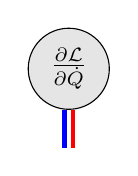
\begin{tikzpicture}[baseline=-.5ex]
        \node[circle,draw,fill=gray!20] (a) at (0,0) {\(\frac{\partial\mathcal{L}}{\partial \dot{Q}}\)};
        \draw[blue, ultra thick, transform canvas={xshift=-1.5pt}] (a) -- +(0,-1);
        \draw[red, ultra thick, transform canvas={xshift=1.5pt}] (a) -- +(0,-1);
    \end{tikzpicture} &= \frac{1}{2}\left(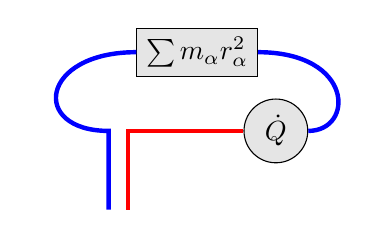
\begin{tikzpicture}[baseline={([yshift=-.5ex]current bounding box.center)}]
        \node (a) at (0,0) {};
        \node[circle,draw,fill=gray!20] (b) at (2,0) {\(\dot{Q}\)};
        \node[draw,fill=gray!20] (c) at (1,1) {\(\sum m_\alpha r_\alpha^2\)};
        \draw[ultra thick, red] (b) -- (a.east) -- +(0,-1);
        \draw[ultra thick, blue] (c) .. controls +(-2,0) and +(-1,0) .. (a.west) -- +(0,-1);
        \draw[ultra thick, blue] (c) .. controls +(2,0) and +(1,0) .. (b);
    \end{tikzpicture} + 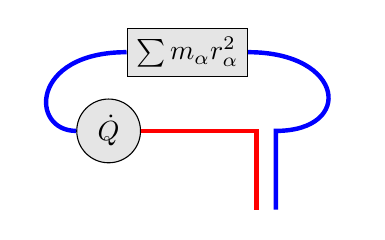
\begin{tikzpicture}[baseline={([yshift=-.5ex]current bounding box.center)}]
        \node[circle,draw,fill=gray!20] (a) at (0,0) {\(\dot{Q}\)};
        \node (b) at (2,0) {};
        \node[draw,fill=gray!20] (c) at (1,1) {\(\sum m_\alpha r_\alpha^2\)};
        \draw[ultra thick, red] (a) -- (b.west) -- +(0,-1);
        \draw[ultra thick, blue] (c) .. controls +(-2,0) and +(-1,0) .. (a);
        \draw[ultra thick, blue] (c) .. controls +(2,0) and +(1,0) .. (b.east) -- +(0,-1);
    \end{tikzpicture}\right)
    \\ &= 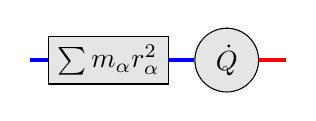
\begin{tikzpicture}[baseline={([yshift=-.5ex]current bounding box.center)}]
        \node[draw,fill=gray!20] (l) at (1,0) {\(\sum m_\alpha r_\alpha^2\)};
        \node[circle,draw,fill=gray!20] (q) at (2.5,0) {\(\dot{Q}\)};
        \draw[ultra thick, blue] (0,0) -- (l) -- (q);
        \draw[ultra thick, red] (q) -- (3.25,0);
    \end{tikzpicture}
    \\ 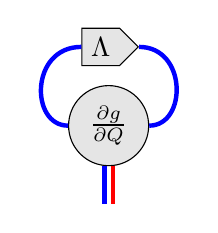
\begin{tikzpicture}[baseline=-.5ex]
        \node[circle,draw,fill=gray!20] (a) at (0,0) {\(\frac{\partial g}{\partial Q}\)};
        \node[signal,draw,fill=gray!20] (l) at (-0.1,1) {\(\Lambda\)};
        \draw[blue, ultra thick, transform canvas={xshift=-1.5pt}] (a) -- +(0,-1);
        \draw[red, ultra thick, transform canvas={xshift=1.5pt}] (a) -- +(0,-1);
        \draw[blue, ultra thick] (a) .. controls (-1,0) and (-1,1) .. (l) .. controls (1,1) and (1,0) .. (a);
    \end{tikzpicture} &= \left(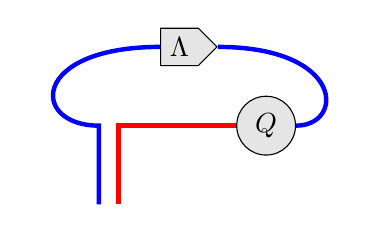
\begin{tikzpicture}[baseline={([yshift=-.5ex]current bounding box.center)}]
        \node (a) at (-1,0) {};
        \node[circle,draw,fill=gray!20] (b) at (1,0) {\(Q\)};
        \node[signal,draw,fill=gray!20] (c) at (-0.1,1) {\(\Lambda\)};
        \draw[ultra thick, red] (b) -- (a.east) -- +(0,-1);
        \draw[ultra thick, blue] (c) .. controls (-2,1) and (-2,0) .. (a.west) -- +(0,-1);
        \draw[ultra thick, blue] (c) .. controls (2,1) and (2,0) .. (b);
    \end{tikzpicture} + 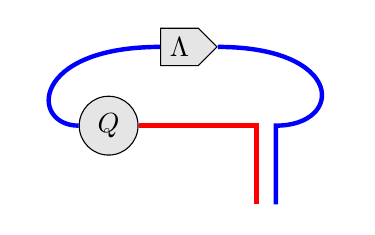
\begin{tikzpicture}[baseline={([yshift=-.5ex]current bounding box.center)}]
        \node[circle,draw,fill=gray!20] (a) at (-1,0) {\(Q\)};
        \node (b) at (1,0) {};
        \node[signal,draw,fill=gray!20] (c) at (-0.1,1) {\(\Lambda\)};
        \draw[ultra thick, red] (a) -- (b.west) -- +(0,-1);
        \draw[ultra thick, blue] (c) .. controls (-2,1) and (-2,0) .. (a);
        \draw[ultra thick, blue] (c) .. controls (2,1) and (2,0) .. (b.east) -- +(0,-1);
    \end{tikzpicture}\right)
    \\ &= 2\left(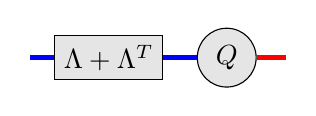
\begin{tikzpicture}[baseline={([yshift=-.5ex]current bounding box.center)}]
        \node[draw,fill=gray!20] (l) at (1,0) {\(\Lambda + \Lambda^T\)};
        \node[circle,draw,fill=gray!20] (q) at (2.5,0) {\(Q\)};
        \draw[ultra thick, blue] (0,0) -- (l) -- (q);
        \draw[ultra thick, red] (q) -- (3.25,0);
    \end{tikzpicture}\right)
\end{align*}

So:
\[
    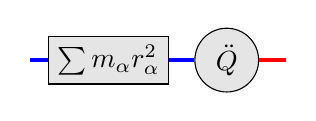
\begin{tikzpicture}[baseline={([yshift=-.5ex]current bounding box.center)}]
        \node[draw,fill=gray!20] (l) at (1,0) {\(\sum m_\alpha r_\alpha^2\)};
        \node[circle,draw,fill=gray!20] (q) at (2.5,0) {\(\ddot{Q}\)};
        \draw[ultra thick, blue] (0,0) -- (l) -- (q);
        \draw[ultra thick, red] (q) -- (3.25,0);
    \end{tikzpicture}
    =
    2\left(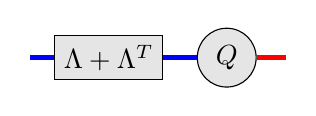
\begin{tikzpicture}[baseline={([yshift=-.5ex]current bounding box.center)}]
        \node[draw,fill=gray!20] (l) at (1,0) {\(\Lambda + \Lambda^T\)};
        \node[circle,draw,fill=gray!20] (q) at (2.5,0) {\(Q\)};
        \draw[ultra thick, blue] (0,0) -- (l) -- (q);
        \draw[ultra thick, red] (q) -- (3.25,0);
    \end{tikzpicture}\right)
\]

In other words:
\[
    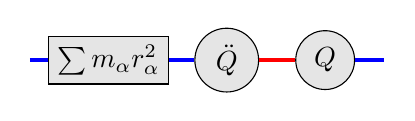
\begin{tikzpicture}[baseline={([yshift=-.5ex]current bounding box.center)}]
        \node[draw,fill=gray!20] (l) at (1,0) {\(\sum m_\alpha r_\alpha^2\)};
        \node[circle,draw,fill=gray!20] (q) at (2.5,0) {\(\ddot{Q}\)};
        \node[circle,draw,fill=gray!20] (q') at (3.75,0) {\(Q\)};
        \draw[ultra thick, blue] (0,0) -- (l) -- (q);
        \draw[ultra thick, red] (q) -- (q');
        \draw[ultra thick, blue] (q') -- (4.5,0);
    \end{tikzpicture}
    =
    2\left(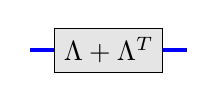
\begin{tikzpicture}[baseline={([yshift=-.5ex]current bounding box.center)}]
        \node[draw,fill=gray!20] (l) at (1,0) {\(\Lambda + \Lambda^T\)};
        \draw[ultra thick, blue] (0,0) -- (l) -- (2,0);
    \end{tikzpicture}\right)
\]

So 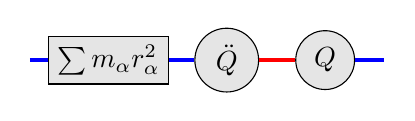
\begin{tikzpicture}[baseline={([yshift=-.5ex]current bounding box.center)}]
    \node[draw,fill=gray!20] (l) at (1,0) {\(\sum m_\alpha r_\alpha^2\)};
    \node[circle,draw,fill=gray!20] (q) at (2.5,0) {\(\ddot{Q}\)};
    \node[circle,draw,fill=gray!20] (q') at (3.75,0) {\(Q\)};
    \draw[ultra thick, blue] (0,0) -- (l) -- (q);
    \draw[ultra thick, red] (q) -- (q');
    \draw[ultra thick, blue] (q') -- (4.5,0);
\end{tikzpicture} is symmetric.

That's the equation of motion.

\pagebreak

Say we want to work in the body frame. Then we'll say the angular velocity is
\(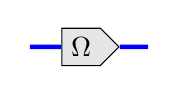
\begin{tikzpicture}[baseline={([yshift=-.5ex]current bounding box.center)}]
    \node[signal,draw,fill=gray!20] (a) at (0.65,0) {\(\Omega\)};
    \draw[ultra thick, blue] (0,0) -- (a) -- (1.5,0);
\end{tikzpicture} = 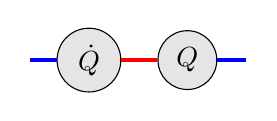
\begin{tikzpicture}[baseline={([yshift=-.5ex]current bounding box.center)}]
    \node[circle,draw,fill=gray!20] (a) at (0.75,0) {\(\dot{Q}\)};
    \node[circle,draw,fill=gray!20] (b) at (2,0) {\(Q\)};
    \draw[ultra thick, blue] (0,0) -- (a);
    \draw[ultra thick, red] (a) -- (b);
    \draw[ultra thick, blue] (b) -- (2.75,0);
\end{tikzpicture}\). This is an antisymmetric matrix, because
\(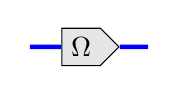
\begin{tikzpicture}[baseline={([yshift=-.5ex]current bounding box.center)}]
    \node[signal,draw,fill=gray!20] (a) at (0.65,0) {\(\Omega\)};
    \draw[ultra thick, blue] (0,0) -- (a) -- (1.5,0);
\end{tikzpicture} + 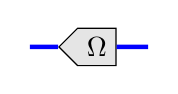
\begin{tikzpicture}[baseline={([yshift=-.5ex]current bounding box.center)}]
    \node[signal, signal to=west,draw,fill=gray!20] (a) at (0.85,0) {\(\Omega\)};
    \draw[ultra thick, blue] (0,0) -- (a) -- (1.5,0);
\end{tikzpicture} = 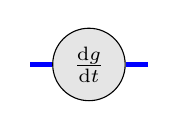
\begin{tikzpicture}[baseline={([yshift=-.5ex]current bounding box.center)}]
    \node[circle,draw,fill=gray!20] (a) at (0,0) {\(\frac{\mathrm{d}g}{\mathrm{d}t}\)};
    \draw[blue, ultra thick] (a) -- (-0.75,0);
    \draw[blue, ultra thick] (a) -- (0.75,0);
\end{tikzpicture} = 0\).

We compute:
\begin{align*}
    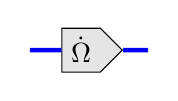
\begin{tikzpicture}[baseline={([yshift=-.5ex]current bounding box.center)}]
        \node[signal,draw,fill=gray!20] (a) at (0.65,0) {\(\dot\Omega\)};
        \draw[ultra thick, blue] (0,0) -- (a) -- (1.5,0);
    \end{tikzpicture} &= 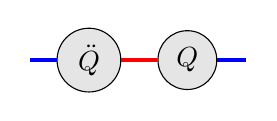
\begin{tikzpicture}[baseline={([yshift=-.5ex]current bounding box.center)}]
        \node[circle,draw,fill=gray!20] (a) at (0.75,0) {\(\ddot{Q}\)};
        \node[circle,draw,fill=gray!20] (b) at (2,0) {\(Q\)};
        \draw[ultra thick, blue] (0,0) -- (a);
        \draw[ultra thick, red] (a) -- (b);
        \draw[ultra thick, blue] (b) -- (2.75,0);
    \end{tikzpicture} + 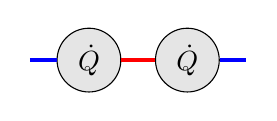
\begin{tikzpicture}[baseline={([yshift=-.5ex]current bounding box.center)}]
        \node[circle,draw,fill=gray!20] (a) at (0.75,0) {\(\dot{Q}\)};
        \node[circle,draw,fill=gray!20] (b) at (2,0) {\(\dot{Q}\)};
        \draw[ultra thick, blue] (0,0) -- (a);
        \draw[ultra thick, red] (a) -- (b);
        \draw[ultra thick, blue] (b) -- (2.75,0);
    \end{tikzpicture}
    \\ &= 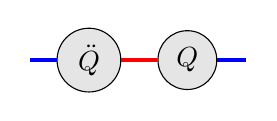
\begin{tikzpicture}[baseline={([yshift=-.5ex]current bounding box.center)}]
        \node[circle,draw,fill=gray!20] (a) at (0.75,0) {\(\ddot{Q}\)};
        \node[circle,draw,fill=gray!20] (b) at (2,0) {\(Q\)};
        \draw[ultra thick, blue] (0,0) -- (a);
        \draw[ultra thick, red] (a) -- (b);
        \draw[ultra thick, blue] (b) -- (2.75,0);
    \end{tikzpicture} + 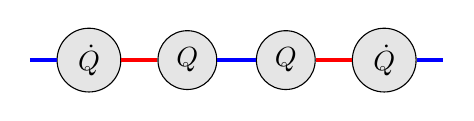
\begin{tikzpicture}[baseline={([yshift=-.5ex]current bounding box.center)}]
        \node[circle,draw,fill=gray!20] (a) at (0.75,0) {\(\dot{Q}\)};
        \node[circle,draw,fill=gray!20] (b) at (2,0) {\(Q\)};
        \node[circle,draw,fill=gray!20] (c) at (3.25,0) {\(Q\)};
        \node[circle,draw,fill=gray!20] (d) at (4.5,0) {\(\dot{Q}\)};
        \draw[ultra thick, blue] (0,0) -- (a);
        \draw[ultra thick, red] (a) -- (b);
        \draw[ultra thick, blue] (b) -- (c);
        \draw[ultra thick, red] (c) -- (d);
        \draw[ultra thick, blue] (d) -- (5.25,0);
    \end{tikzpicture}
    \\ &= 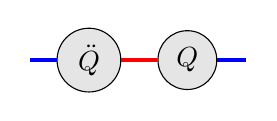
\begin{tikzpicture}[baseline={([yshift=-.5ex]current bounding box.center)}]
        \node[circle,draw,fill=gray!20] (a) at (0.75,0) {\(\ddot{Q}\)};
        \node[circle,draw,fill=gray!20] (b) at (2,0) {\(Q\)};
        \draw[ultra thick, blue] (0,0) -- (a);
        \draw[ultra thick, red] (a) -- (b);
        \draw[ultra thick, blue] (b) -- (2.75,0);
    \end{tikzpicture} + 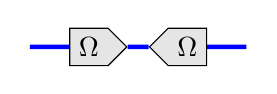
\begin{tikzpicture}[baseline={([yshift=-.5ex]current bounding box.center)}]
        \node[signal,draw,fill=gray!20] (a) at (0.75,0) {\(\Omega\)};
        \node[signal, signal to=west,draw,fill=gray!20] (b) at (2,0) {\(\Omega\)};
        \draw[ultra thick, blue] (0,0) -- (a) -- (b) -- (2.75,0);
    \end{tikzpicture}
    \\ &= 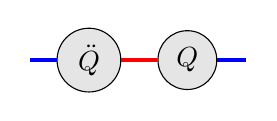
\begin{tikzpicture}[baseline={([yshift=-.5ex]current bounding box.center)}]
        \node[circle,draw,fill=gray!20] (a) at (0.75,0) {\(\ddot{Q}\)};
        \node[circle,draw,fill=gray!20] (b) at (2,0) {\(Q\)};
        \draw[ultra thick, blue] (0,0) -- (a);
        \draw[ultra thick, red] (a) -- (b);
        \draw[ultra thick, blue] (b) -- (2.75,0);
    \end{tikzpicture} - 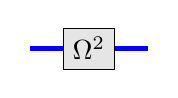
\begin{tikzpicture}[baseline={([yshift=-.5ex]current bounding box.center)}]
        \node[draw,fill=gray!20] (a) at (0.75,0) {\(\Omega^2\)};
        \draw[ultra thick, blue] (0,0) -- (a) -- (1.5,0);
    \end{tikzpicture}
    \\ 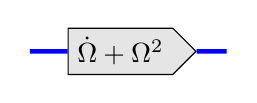
\begin{tikzpicture}[baseline={([yshift=-.5ex]current bounding box.center)}]
        \node[signal,draw,fill=gray!20] (a) at (1.15,0) {\(\dot\Omega + \Omega^2\)};
        \draw[ultra thick, blue] (0,0) -- (a) -- (2.5,0);
    \end{tikzpicture} &= 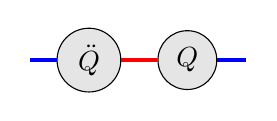
\begin{tikzpicture}[baseline={([yshift=-.5ex]current bounding box.center)}]
        \node[circle,draw,fill=gray!20] (a) at (0.75,0) {\(\ddot{Q}\)};
        \node[circle,draw,fill=gray!20] (b) at (2,0) {\(Q\)};
        \draw[ultra thick, blue] (0,0) -- (a);
        \draw[ultra thick, red] (a) -- (b);
        \draw[ultra thick, blue] (b) -- (2.75,0);
    \end{tikzpicture}
\end{align*}

So 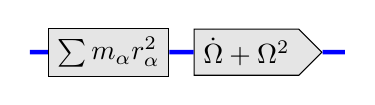
\begin{tikzpicture}[baseline={([yshift=-.5ex]current bounding box.center)}]
    \node[draw,fill=gray!20] (a) at (1,0) {\(\sum m_\alpha r_\alpha^2\)};
    \node[signal,draw,fill=gray!20] (b) at (2.75,0) {\(\dot\Omega + \Omega^2\)};
    \draw[ultra thick, blue] (0,0) -- (a) -- (b) -- (4,0);
\end{tikzpicture} is symmetric.

\vspace*{1em}\hrule\vspace*{1em}

If we want, we can solve for \(\dot\Omega\).

\begin{align*}
    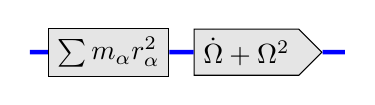
\begin{tikzpicture}[baseline={([yshift=-.5ex]current bounding box.center)}]
        \node[draw,fill=gray!20] (a) at (1,0) {\(\sum m_\alpha r_\alpha^2\)};
        \node[signal,draw,fill=gray!20] (b) at (2.75,0) {\(\dot\Omega + \Omega^2\)};
        \draw[ultra thick, blue] (0,0) -- (a) -- (b) -- (4,0);
    \end{tikzpicture} &= 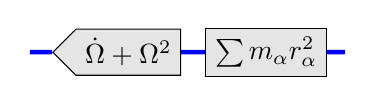
\begin{tikzpicture}[baseline={([yshift=-.5ex]current bounding box.center)}]
        \node[signal, signal to=west,draw,fill=gray!20] (a) at (1.25,0) {\(\dot\Omega + \Omega^2\)};
        \node[draw,fill=gray!20] (b) at (3,0) {\(\sum m_\alpha r_\alpha^2\)};
        \draw[ultra thick, blue] (0,0) -- (a) -- (b) -- (4,0);
    \end{tikzpicture}
    \\ &= 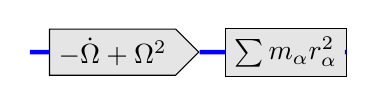
\begin{tikzpicture}[baseline={([yshift=-.5ex]current bounding box.center)}]
        \node[signal,draw,fill=gray!20] (a) at (1.05,0) {\(-\dot\Omega + \Omega^2\)};
        \node[draw,fill=gray!20] (b) at (3.25,0) {\(\sum m_\alpha r_\alpha^2\)};
        \draw[ultra thick, blue] (0,0) -- (a) -- (b) -- (4,0);
    \end{tikzpicture}
    \\ 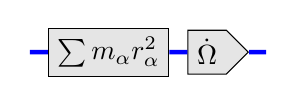
\begin{tikzpicture}[baseline={([yshift=-.5ex]current bounding box.center)}]
        \node[draw,fill=gray!20] (a) at (1,0) {\(\sum m_\alpha r_\alpha^2\)};
        \node[signal,draw,fill=gray!20] (b) at (2.25,0) {\(\dot\Omega\)};
        \draw[ultra thick, blue] (0,0) -- (a) -- (b) -- (3,0);
    \end{tikzpicture} + 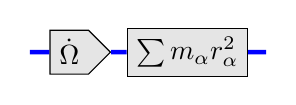
\begin{tikzpicture}[baseline={([yshift=-.5ex]current bounding box.center)}]
        \node[signal,draw,fill=gray!20] (a) at (0.5,0) {\(\dot\Omega\)};
        \node[draw,fill=gray!20] (b) at (2,0) {\(\sum m_\alpha r_\alpha^2\)};
        \draw[ultra thick, blue] (0,0) -- (a) -- (b) -- (3,0);
    \end{tikzpicture} &= 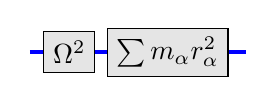
\begin{tikzpicture}[baseline={([yshift=-.5ex]current bounding box.center)}]
        \node[draw,fill=gray!20] (a) at (0.5,0) {\(\Omega^2\)};
        \node[draw,fill=gray!20] (b) at (1.75,0) {\(\sum m_\alpha r_\alpha^2\)};
        \draw[ultra thick, blue] (0,0) -- (a) -- (b) -- (2.75,0);
    \end{tikzpicture} - 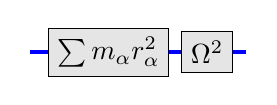
\begin{tikzpicture}[baseline={([yshift=-.5ex]current bounding box.center)}]
        \node[draw,fill=gray!20] (a) at (1,0) {\(\sum m_\alpha r_\alpha^2\)};
        \node[draw,fill=gray!20] (b) at (2.25,0) {\(\Omega^2\)};
        \draw[ultra thick, blue] (0,0) -- (a) -- (b) -- (2.75,0);
    \end{tikzpicture}
    \\ \begin{tikzpicture}[baseline={([yshift=-.5ex]current bounding box.center)}]
        \node[draw,fill=gray!20] (i) at (0,1) {\(\left(\sum m_\alpha r_\alpha^2\right) \otimes \mathrm{id} + \mathrm{id} \otimes \left(\sum m_\alpha r_\alpha^2\right)\)};
        \node[signal,draw,fill=gray!20] (a) at (0,0) {\(\dot\Omega\)};
        \draw[ultra thick, blue] ($(a.north)+(0.1,0)$) -- ($(i.south)+(0.1,0)$);
        \draw[ultra thick, blue] ($(a.north)+(-0.1,0)$) -- ($(i.south)+(-0.1,0)$);
        \draw[ultra thick, blue] ($(i.north)+(0.1,0)$) -- (0.1,2);
        \draw[ultra thick, blue] ($(i.north)+(-0.1,0)$) -- (-0.1,2);
    \end{tikzpicture} &= \begin{tikzpicture}[baseline={([yshift=-.5ex]current bounding box.center)}]
        \node[draw,fill=gray!20] (i) at (0,1) {\(-\left(\sum m_\alpha r_\alpha^2\right) \otimes \mathrm{id} + \mathrm{id} \otimes \left(\sum m_\alpha r_\alpha^2\right)\)};
        \node[draw,fill=gray!20] (a) at (0,0) {\(\Omega^2\)};
        \draw[ultra thick, blue] ($(a.north)+(0.1,0)$) -- ($(i.south)+(0.1,0)$);
        \draw[ultra thick, blue] ($(a.north)+(-0.1,0)$) -- ($(i.south)+(-0.1,0)$);
        \draw[ultra thick, blue] ($(i.north)+(0.1,0)$) -- (0.1,2);
        \draw[ultra thick, blue] ($(i.north)+(-0.1,0)$) -- (-0.1,2);
    \end{tikzpicture}
\end{align*}

The big box on the left, treated as a map from antisymmetric matrices to antisymmetric matrices, is the inertia tensor \(I\).
It is invertible in a suitable sense, so we get an equation for \(\dot\Omega\).

\[\begin{tikzpicture}[baseline=-.5ex]
    \node[signal,draw,fill=gray!20] (a) at (0,0) {\(\dot\Omega\)};
    \draw[ultra thick, blue] ($(a.north)+(0.1,0)$) -- (0.1,0.5);
    \draw[ultra thick, blue] ($(a.north)+(-0.1,0)$) -- (-0.1,0.5);
\end{tikzpicture} = \begin{tikzpicture}[baseline=-.5ex]
    \node[draw,fill=gray!20] (i) at (0,0.75) {\(I^{-1}\)};
    \node[draw,fill=gray!20] (i') at (0,0) {\(-\left(\sum m_\alpha r_\alpha^2\right) \otimes \mathrm{id} + \mathrm{id} \otimes \left(\sum m_\alpha r_\alpha^2\right)\)};
    \node[draw,fill=gray!20] (a) at (0,-0.75) {\(\Omega^2\)};
    \draw[ultra thick, blue] ($(a.north)+(0.1,0)$) -- ($(i'.south)+(0.1,0)$);
    \draw[ultra thick, blue] ($(a.north)+(-0.1,0)$) -- ($(i'.south)+(-0.1,0)$);
    \draw[ultra thick, blue] ($(i'.north)+(0.1,0)$) -- ($(i.south)+(0.1,0)$);
    \draw[ultra thick, blue] ($(i'.north)+(-0.1,0)$) -- ($(i.south)+(-0.1,0)$);
    \draw[ultra thick, blue] ($(i.north)+(0.1,0)$) -- (0.1,1.25);
    \draw[ultra thick, blue] ($(i.north)+(-0.1,0)$) -- (-0.1,1.25);
\end{tikzpicture}\]

\pagebreak

Let's work in a convenient basis.
\[\sum m_\alpha r_\alpha^2 = \begin{bmatrix}
    a_0 \\ & a_1 \\ && a_2 \\ &&& a_3 \\ &&&& \ddots
\end{bmatrix}\]

Then this formula simplifies. We compute:

\begin{align*}
    \begin{tikzpicture}[baseline=-.5ex]
        \node[draw,fill=gray!20] (i) at (0,0) {\(\left(\sum m_\alpha r_\alpha^2\right) \otimes \mathrm{id} + \mathrm{id} \otimes \left(\sum m_\alpha r_\alpha^2\right)\)};
        \node[signal,draw,fill=gray!20] (a) at (0,-0.75) {\(e_i \otimes e_j - e_j \otimes e_i\)};
        \draw[ultra thick, blue] ($(a.north)+(0.1,0)$) -- ($(i.south)+(0.1,0)$);
        \draw[ultra thick, blue] ($(a.north)+(-0.1,0)$) -- ($(i.south)+(-0.1,0)$);
        \draw[ultra thick, blue] ($(i.north)+(0.1,0)$) -- (0.1,0.5);
        \draw[ultra thick, blue] ($(i.north)+(-0.1,0)$) -- (-0.1,0.5);
    \end{tikzpicture}
    &= \begin{tikzpicture}[baseline=-.5ex]
        \node[signal,draw,fill=gray!20] (a) at (0,0) {\((a_i + a_j)(e_i \otimes e_j - e_j \otimes e_i)\)};
        \draw[ultra thick, blue] ($(a.north)+(0.1,0)$) -- (0.1,0.5);
        \draw[ultra thick, blue] ($(a.north)+(-0.1,0)$) -- (-0.1,0.5);
    \end{tikzpicture}
    \\ \begin{tikzpicture}[baseline=-.5ex]
        \node[draw,fill=gray!20] (i) at (0,0) {\(-\left(\sum m_\alpha r_\alpha^2\right) \otimes \mathrm{id} + \mathrm{id} \otimes \left(\sum m_\alpha r_\alpha^2\right)\)};
        \node[signal,draw,fill=gray!20] (a) at (0,-0.75) {\(e_i \otimes e_j + e_j \otimes e_i\)};
        \draw[ultra thick, blue] ($(a.north)+(0.1,0)$) -- ($(i.south)+(0.1,0)$);
        \draw[ultra thick, blue] ($(a.north)+(-0.1,0)$) -- ($(i.south)+(-0.1,0)$);
        \draw[ultra thick, blue] ($(i.north)+(0.1,0)$) -- (0.1,0.5);
        \draw[ultra thick, blue] ($(i.north)+(-0.1,0)$) -- (-0.1,0.5);
    \end{tikzpicture}
    &= \begin{tikzpicture}[baseline=-.5ex]
        \node[signal,draw,fill=gray!20] (a) at (0,0) {\((a_j - a_i)(e_i \otimes e_j - e_j \otimes e_i)\)};
        \draw[ultra thick, blue] ($(a.north)+(0.1,0)$) -- (0.1,0.5);
        \draw[ultra thick, blue] ($(a.north)+(-0.1,0)$) -- (-0.1,0.5);
    \end{tikzpicture}
\end{align*}

\[\dot{\Omega}_{ij} = \frac{a_j - a_i}{a_i + a_j} (\Omega^2)_{ij}\]

\vspace*{1em}\hrule\vspace*{1em}

It is clear, then, that if the body is fully asymmetric, then equilibrium occurs when \(\Omega^2\) is diagonal.
If \(\Omega\)'s eigenvalues are likewise maximally distinct, then we have, up to permuting rows and columns:
\begin{align*}
    \Omega &= \begin{bmatrix}
        &&&&\omega_0 \\ &&&\omega_1 \\ &&\reflectbox{$\ddots$} \\ &\omega_{n-1} \\ \omega_n
    \end{bmatrix}
    \\ &\text{(where \(\omega_k = -\omega_{n-k}\)).}
\end{align*}

That is, the planes of rotation are spanned by pairs of principal axes.

\vspace*{1em}\hrule\vspace*{1em}

When is the equilibrium stable? Linearize by setting \(\Omega = \Omega_0 + \epsilon\Omega_1\), where \(\Omega_0\) is an equilibrium, and take the order \(\epsilon\) part.
\begin{align*}
    (\dot{\Omega}_1)_{ij} &= \frac{a_j - a_i}{a_i + a_j} (\Omega_0\Omega_1 + \Omega_1\Omega_0)_{ij}
    \\ &= \frac{a_j - a_i}{a_i + a_j} (\omega_i (\Omega_1)_{(n-i)j} + \omega_{n-j}(\Omega_1)_{i(n-j)})
\end{align*}

For any \(i\) and \(j\), this linear transformation \(\Omega_1 \mapsto \dot\Omega_1\) preserves the subspace of matrices which are nonzero only when both indices are either \(i\), \(j\), \(n-i\), or \(n-j\).
We'll find all our eigenvectors in those subspaces. So, in essence, \emph{we can reduce the problem to the case where there are only four dimensions.}

\pagebreak

Let's work in four dimensions. Then \(\Omega_1\) is a six-dimensional vector:
\[\begin{bmatrix}
    (\Omega_1)_{01} \\ (\Omega_1)_{02} \\ (\Omega_1)_{03} \\ (\Omega_1)_{12} \\ (\Omega_1)_{13} \\ (\Omega_1)_{23}
\end{bmatrix}\]

The linearized equations of motion are thus given by a \(6 \times 6\) matrix.
\[\dot\Omega_1 = \begin{bmatrix}
    0 & \frac{a_1 - a_0}{a_0 + a_1}\omega_2 & 0 & 0 & -\frac{a_1 - a_0}{a_0 + a_1}\omega_0 & 0 \\
    \frac{a_2 - a_0}{a_0 + a_2}\omega_1 & 0 & 0 & 0 & 0 & -\frac{a_2 - a_0}{a_0 + a_2}\omega_0 \\
    0 & 0 & 0 & 0 & 0 & 0 \\
    0 & 0 & 0 & 0 & 0 & 0 \\
    -\frac{a_3 - a_1}{a_1 + a_3}\omega_0 & 0 & 0 & 0 & 0 & \frac{a_3 - a_1}{a_1 + a_3}\omega_1 \\
    0 & -\frac{a_3 - a_2}{a_2 + a_3}\omega_0 & 0 & 0 & \frac{a_3 - a_2}{a_2 + a_3}\omega_2 & 0 \\
\end{bmatrix}\Omega_1\]

Simplifying using \(\omega_2 = -\omega_1\):
\[\dot\Omega_1 = \begin{bmatrix}
    0 & -\frac{a_1 - a_0}{a_0 + a_1}\omega_1 & 0 & 0 & -\frac{a_1 - a_0}{a_0 + a_1}\omega_0 & 0 \\
    \frac{a_2 - a_0}{a_0 + a_2}\omega_1 & 0 & 0 & 0 & 0 & -\frac{a_2 - a_0}{a_0 + a_2}\omega_0 \\
    0 & 0 & 0 & 0 & 0 & 0 \\
    0 & 0 & 0 & 0 & 0 & 0 \\
    -\frac{a_3 - a_1}{a_1 + a_3}\omega_0 & 0 & 0 & 0 & 0 & \frac{a_3 - a_1}{a_1 + a_3}\omega_1 \\
    0 & -\frac{a_3 - a_2}{a_2 + a_3}\omega_0 & 0 & 0 & -\frac{a_3 - a_2}{a_2 + a_3}\omega_1 & 0 \\
\end{bmatrix}\Omega_1\]

To simplify, define \(\alpha = \frac{a_1 - a_0}{a_0 + a_1}\), \(\beta = \frac{a_2 - a_0}{a_0 + a_2}\), \(\gamma = \frac{a_3 - a_1}{a_1 + a_3}\), and \(\delta = \frac{a_3 - a_2}{a_2 + a_3}\).

\[\dot\Omega_1 = \begin{bmatrix}
    0 & -\alpha\omega_1 & 0 & 0 & -\alpha\omega_0 & 0 \\
    \beta\omega_1 & 0 & 0 & 0 & 0 & -\beta\omega_0 \\
    0 & 0 & 0 & 0 & 0 & 0 \\
    0 & 0 & 0 & 0 & 0 & 0 \\
    -\gamma\omega_0 & 0 & 0 & 0 & 0 & \gamma\omega_1 \\
    0 & -\delta\omega_0 & 0 & 0 & -\delta\omega_1 & 0 \\
\end{bmatrix}\Omega_1\]

% \pagebreak

We drop the trivial rows and columns, then compute the characteristic polynomial.

\begin{align*}
    &\det \begin{bmatrix}
        -\lambda & (-\alpha)\omega_1 & (-\alpha)\omega_0 & \\
        (\beta)\omega_1 & -\lambda & & (-\beta)\omega_0 \\
        (-\gamma)\omega_0 & & -\lambda & (\gamma)\omega_1 \\
        & (-\delta)\omega_0 & (-\delta)\omega_1 & -\lambda \\
    \end{bmatrix}
    \\ &= \lambda^4 - (-\delta)(\gamma) \lambda^2\omega_1^2 - (-\delta)(-\beta) \lambda^2\omega_0^2
    \\ &- (\beta)(-\alpha)\lambda^2\omega_1^2 + (\beta)(-\alpha)(-\delta)(\gamma) \omega_1^4 - (\beta)(-\delta)(-\alpha)(\gamma)\omega_0^2\omega_1^2
    \\ &- (-\gamma)(-\alpha)(-\delta)(-\beta)\omega_0^2\omega_1^2 - (-\gamma)(-\alpha)\omega_0^2\lambda^2 + (-\gamma)(-\delta)(-\alpha)(-\beta)\omega_0^4
    \\ &= \lambda^4 + ((\alpha\beta + \gamma\delta)\omega_1^2 - (\alpha\gamma + \beta\delta) \omega_0^2)\lambda^2 + \alpha\beta\gamma\delta (\omega_1^2 - \omega_0^2)^2
\end{align*}

\pagebreak

I have not yet found a clean-enough way to determine when the roots are all imaginary.

\end{document}